\section{Begriffe und Elemente}

\subsection{Akteur}

Ein \textbf{Akteur} ist ein Anwender {bzw.} ein \textit{externes System}, der mit dem zu betrachtenden System interagiert.\\

\noindent
Akteure befinden sich \textit{außerhalb} des betrachteten Systems und spiegeln \textit{Rollen} wider, \textit{keine} konkreten Personen.


\subsection{Anwendungsfälle}
\textbf{Anwendungsfälle} stellen das \textit{Verhalten} des Systems dar und ermöglichen \textbf{Interaktionen} mit einem oder mehreren \textbf{Akteuren}.\\

\noindent
Anwendungsfälle geben \textiut{keine} Auskunft über \textit{interne Strukturen}.\\
I.d.R. repräsentieren sie einen Dienst nach außen.\\

\begin{tcolorbox}
Anwendungsfälle beschreiben das Szenario der Nutzung, und sind deshalb \textit{nicht} mit einem \textbf{Feature} des Systems zu verwechseln: Features ermöglichen das Szenario, werden aber nicht durch die Anwendungsfälle beschrieben.
\end{tcolorbox}


\subsection{Assoziationsbeziehungen}

\begin{tcolorbox}
\textbf{Assoziationsbeziehungen} können zwischen einem Akteur und einem oder mehreren Anwendungsfällen modelliert werden.
\end{tcolorbox}

\noindent
\textit{Buhl} weist darauf hin, dass bei den Assoziationsbeziehungen grundsätzlich dieselben Aussagen wie in Abschnitt~\ref{sec:klassendiagramme-begriffe-und-elemente} getroffen werden können (vgl. ~\cite[52]{Buh09}).\\

\noindent
In Anwendungsfalldiagrammen \textit{müssen} die Systemgrenzen modelliert werden (vgl.~\cite[52]{Buh09}).\\
Systeme realisieren das Verhalten von Anwendungsfällen, bei denen sich Akteure immer außerhalb des Systems befinden: Entsprechende Systemgrenzen werden als Kasten dargestellt, in dem sich  die Anwendungsfälle befinden.

\subsection{Generalisierungsbeziehungen}
Zwischen Akteuren und Anwendungsfällen können \textbf{Generalisierungsbeziehungen} modelliert werden (vgl. im Folgenden~\cite[66]{Bal05}):

\begin{itemize}
    \item zwischen \textbf{Akteuren}
    \begin{itemize}
        \item Das Verhalten und die Beziehungen zu den Akteuren wird vererbt.
        \item Der spezialisierte Akteur erbt die Eigenschaften des allgemeineren Akteurs und kann weitere Eigenschaften hinzufügen.
    \end{itemize}
    \item zwischen \textbf{Anwendungsfällen}:
    \begin{itemize}
        \item Der spezialisierte Use-Case erbt die Eigenschaften des allgemeineren Use-Cases.
        \item Die Beziehungen des allgemeineren Use-Cases (bspw. \code{extend}-Beziehungen) und seine Assoziationen zu Akteuren werden an die spezialisierten Use-Cases vererbt.
        \item Der spezialisierte Use-Case kann neue Eigenschaften und neues Verhalten definieren.
    \end{itemize}
\end{itemize}

\noindent
Es kann auch eine alternative Darstellung mit dem Klassensymbol verwendet werden, wobei diese Darstellung das Bereitstellen von Zusatzinformation ermöglicht (s. Abbildung~\ref{fig:usecase-notation}).


\begin{figure}
    \centering
    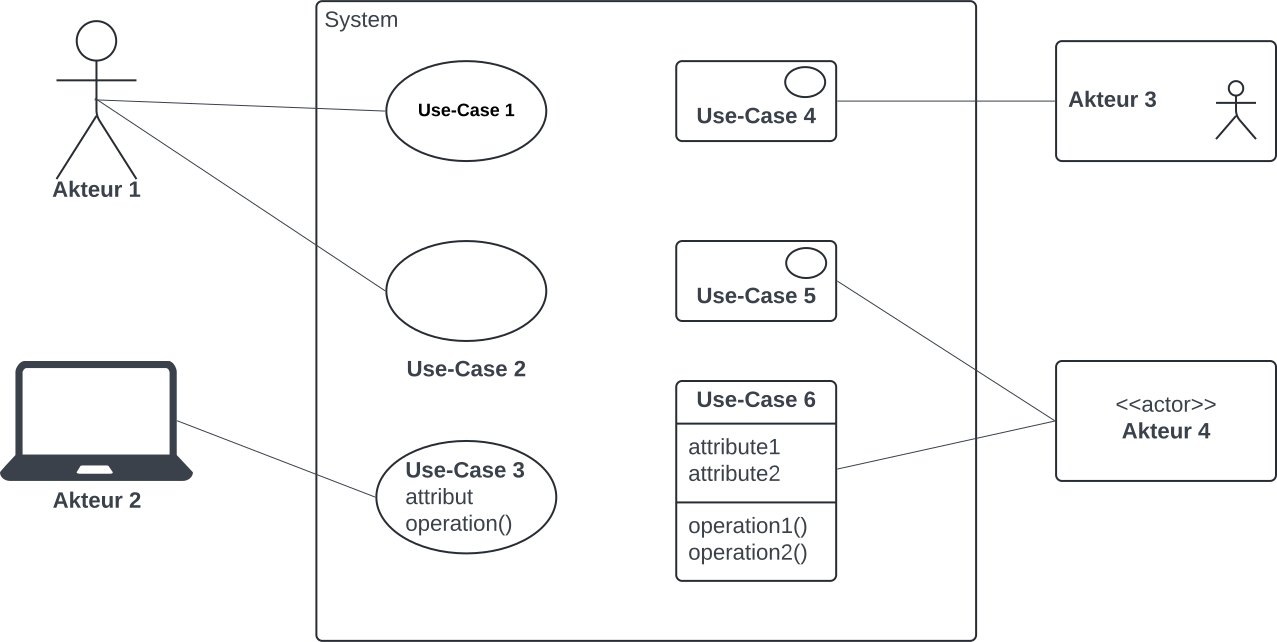
\includegraphics[scale=0.35]{part three/Anwendungsfalldiagramm/img/usecase-notation}
    \caption{Verschiedene Notationen für Elemente in einem Anwendungsfalldiagramm. Bei der Verwendung der Klassennotation wird ein Use-Case-Piktogramm in die rechte obere Ecke gesetzt (vgl.~\cite[63 f.]{Bal05}). (Quelle: in Anlehnung an \cite[64, Abb. 2.8-2]{Bal05})}
    \label{fig:usecase-notation}
\end{figure}


\subsection{include-Beziehung}

Die Modellierung einer \code{include}-Beziehung erlaubt das Wiederverwenden von Verhalten.\\

\noindent
Eine \code{include}-Beziehung dient der Ausgliederung von \textbf{redundantem Verhalten} (s. Abbildung~\ref{fig:usecase-include}).\\

\noindent
Bei der Verwendung einer \code{include}-Beziehung gilt (vgl.~\cite[53]{Buh09}):


\begin{itemize}
    \item es handelt sich um eine \textit{gerichtete} Beziehung zwischen zwei Anwendungsfällen
    \item der inkludierende Anwendungsfall fügt das Verhalten des eingefügten Anwendungsfalls in sein eigenes ein
    \item inkludieren ist \textit{nicht} optional, d.h., der inkludierte Use-Case wird immer für die Ausführung des inkludierenden Use-Cases benötigt (vgl.~\cite[65 f.]{Bal05})
    \item die Ausführung des inkludierten Use-Case ist von keiner Bedingung abhängig
\end{itemize}

\begin{figure}
    \centering
    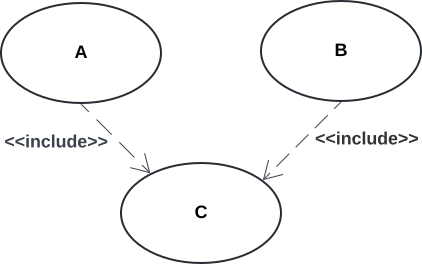
\includegraphics[scale=0.4]{part three/Anwendungsfalldiagramm/img/usecase-include}
    \caption{Notation der include-Beziehung. Die Anwendungsfälle \textbf{A} und \textbf{B} verwenden beide den Anwendungsfall \textbf{C}. (Quelle: in Anlehnung an \cite[66, Abb. 2.8-5]{Bal05})}
    \label{fig:usecase-include}
\end{figure}


\subsection{extend-Beziehung}
Die Verwendung der \code{extend}-Beziehung erlaubt die Erweiterung eines Anwendungsfalles \code{A} durch einen Anwendungsfall \code{B}.\\
\code{A} beschreibt die Basisfunktionalität, \code{B} beschreibt die Erweiterung (s. Abbildung~\ref{fig:usecase-extend}).
Hierbei kann der \textbf{A} alleine oder zusammen mit \code{B} ausgeführt werden (im Unterschied zur \code{include}-Beziehung: Hier ist inkludieren nicht optional) (vgl.~\cite[54]{Bal05}).

\noindent
Bei der Verwendung einer \code{extend}-Beziehung gilt (vgl.~\cite[53]{Buh09}):

\begin{itemize}
    \item das Verhalten eines Anwendungsfalles kann durch das Verhalten eines anderen erweitert werden
    \item die Beziehung zwischen den beteiligten Anwendungsfällen ist gerichtet
    \item spezifische Erweiterungspunkte (\textit{extension points}\footnote{
        ``ExtensionPoints may be listed in a compartment of the UseCase with the heading \textbf{extension points}.`` (\cite[642, Hervorhebung i.O.]{OMG17})
    }) geben an, an welchen Stellen der Basis-Anwendungsfall erweitert wird
    \item Bedingungen zum Auslösen des erweiterten Verhalten wird mit angefügten Notizen spezifiziert
\end{itemize}

\begin{figure}
    \centering
    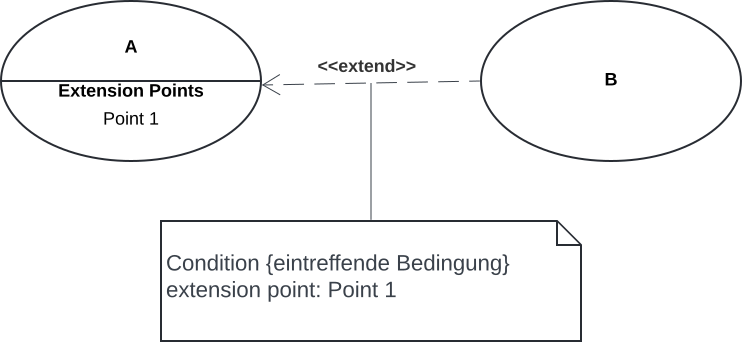
\includegraphics[scale=0.4]{part three/Anwendungsfalldiagramm/img/usecase-extend}
    \caption{Notation der extend-Beziehung. in dem Beispiel wird die der Anwendungsfall \textbf{A} durch den Anwendungsfall \textbf{B} an dem \textit{extension point} \textbf{Point 1} erweitert, der aktiviert wird, falls die in der Notiz vermerkte Bedingung zutrifft (Quelle: in Anlehnung an \cite[65, Abb. 2.8-4]{Bal05})}
    \label{fig:usecase-extend}
\end{figure}

\subsection*{Anmerkung}
Bei der \code{include}-Beziehung zeigt der Pfeil auf den einzubindenden Anwendungsfall.\\
Bei der \code{extend}-Beziehung ist es umgekehrt, der Pfeil zeigt auf den zu erweiternden Anwendungsfall (\cite[218]{Oes05}).